\subsection{Problematiza\c c\~ao da Revis\~ao} \label{subsec: problematização da revisão}

Nesta subseção, é discutido um problema de pesquisa que pode ser compreendido por diversos leitores. A Figura \ref{fig:serie-temporal} apresenta um mapa conceitual das publicações, destacando a importância dos autores como base para esta revisão. Os modelos propostos por esses autores são fundamentais para abordar o problema em questão, uma vez que a previsão em séries temporais é um desafio de grande significado por si só.

\begin{figure}[htb!]
	\centering
	\caption{Fluxograma do problema de pesquisa}
	\label{fig:serie-temporal}
	\includegraphics[width=1\linewidth]{Revisao/Figuras/"Série temporal"}
	
	\fonte{Elaboração própria} 
\end{figure}

O mapa conceitual apresentado na Figura \ref{fig:serie-temporal} ilustra a relação entre as palavras-chave que está relacionada ao problema em questão, proporcionando uma visão clara do que será abordado ao longo do trabalho. Esse mapa contribui para a identificação dos principais tópicos de pesquisa e das questões que serão exploradas posteriormente.

As questões de pesquisa definidas para esta revisão sistemática da literatura são as seguintes:

\begin{enumerate}[start=1, label = {\textbf{Q} \arabic*} ]
	\item \label{questão:rev1} Quais são os autores que mais publicam sobre o assunto de séries temporais?
	\item \label{questão:rev2} Quais são os países que mais publicam sobre o assunto? 
	\item \label{questão:rev3} Quais são as áreas que mais publicam sobre o tema?
	\item \label{questão:rev4} Quais são as obras mais influentes na análise de séries temporais?
\end{enumerate}

Essas questões guiarão a análise e a seleção dos artigos a serem revisados, permitindo uma compreensão mais aprofundada da produção científica relacionada ao tema das séries temporais.

\subsection{Metodologia}\label{subsec:met da revisão}

Nesta subseção, é fornecida uma explicação detalhada de como a revisão foi conduzida, abrangendo desde a análise do banco de dados até a conclusão final da revisão. São apresentados os passos e critérios adotados para a seleção dos artigos, bem como os procedimentos utilizados para a extração e análise dos dados. A subseção visa esclarecer de forma clara e objetiva todo o processo metodológico empregado durante a realização da revisão.

\begin{figure}[!htb]
	\centering
	\caption{Etapas da Revisão}
	\label{fig:rsl}
	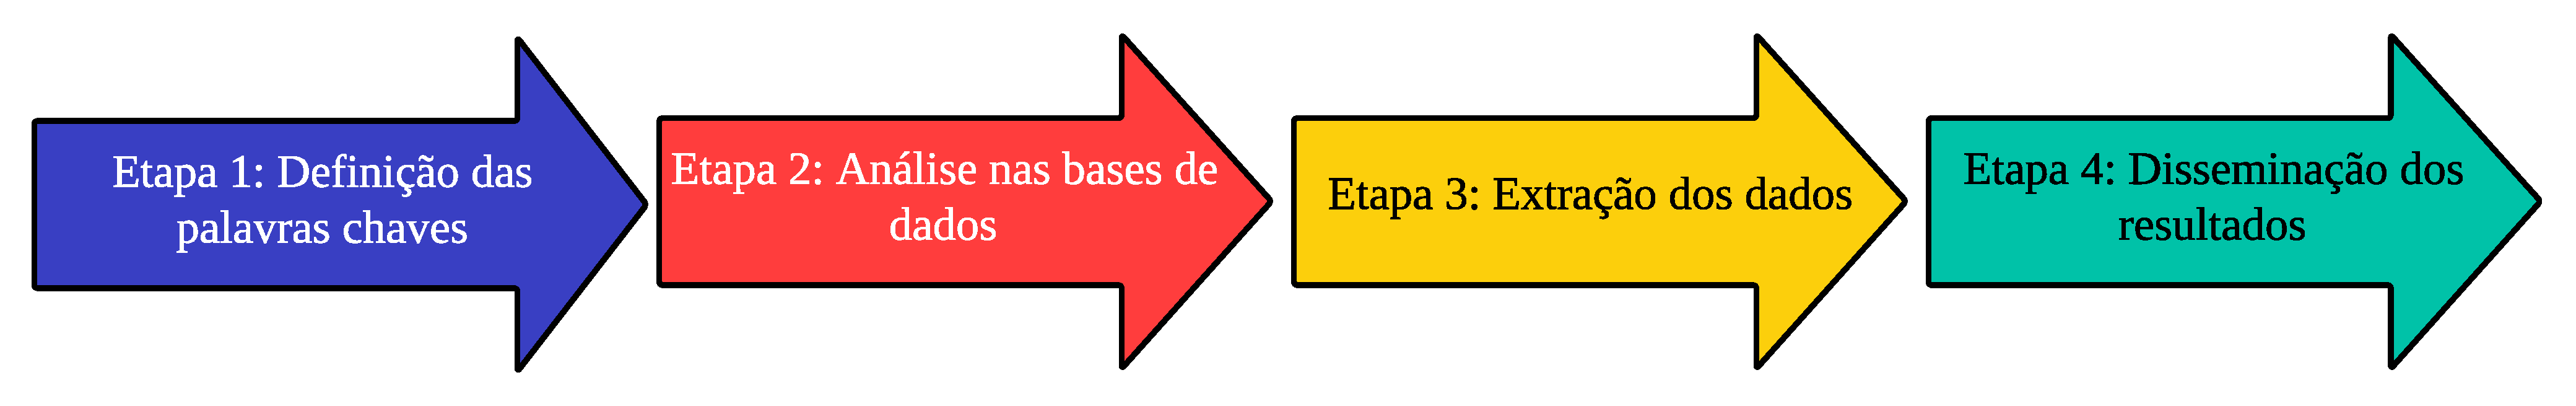
\includegraphics[width=1\linewidth]{Revisao/Figuras/RSL}
	
	\fonte{Adaptado de \citeonline{MARTINS201671}}
\end{figure}


\begin{enumerate}[start=1, label={\textbf{Etapa} \arabic*}]
	
\item \label{etp:rev-1} A Figura \ref{fig:rsl} apresenta uma adaptação da metodologia proposta por \citeonline{MARTINS201671} para a realização desta revisão sistemática. Inicialmente, foram realizadas buscas nos bancos de dados Scopus, Web of Science e Lens, selecionando algumas bases relevantes para o tema da pesquisa.

Para todas as bases de busca, foram considerados os últimos 6 anos, com exceção do Lens, que retornava poucos artigos. Nessa etapa, foram utilizadas palavras-chave que se adequam melhor à pesquisa, como ``\textit{time series forecasting}'', ``\textit{time series analysis}'' e ``\textit{nonlinear forecasting}''.

\item \label{etp:rev-2} No cruzamento das palavras-chave, obteve-se um número considerável de artigos, sem restringir a área em que cada um pode ser publicado. A Tabela \ref{tb1} apresenta a tabulação dos resultados obtidos, sem excluir duplicatas, que serão tratadas na seção \ref{subesec:resul da revisão}.

\item \label{etp:rev-3} Na etapa seguinte, é realizada uma avaliação preliminar de cada artigo obtido, sem aplicar nenhum filtro anual nas buscas. Analisar todos os artigos dessa maneira resultaria em um número elevado, por exemplo, no banco de dados Scopus são 498 artigos, na Web of Science são 140 artigos e no Lens, que retorna poucos artigos, são 11 artigos, totalizando 649 artigos sem remover duplicatas. É importante ressaltar que esses artigos passaram apenas pelo filtro de idioma inglês e de serem artigos, visando aprimorar a busca e a tomada de decisões. Ao aplicar o filtro dos últimos 6 anos, obtém-se um número mais gerenciável de artigos para análise. Levando em consideração a diferença entre essa estimativa apresentada na Tabela \ref{tb1} e a quantidade de artigos restantes após a remoção de duplicatas, tem-se menos de 356 artigos para análise. É válido lembrar que, ao remover as duplicatas, esse número pode diminuir ainda mais, atingindo o objetivo proposto neste trabalho.

\item \label{etp:rev-4} Na etapa final, é realizada uma análise mais aprofundada do conteúdo dos artigos selecionados, levando em consideração as áreas de especialização e correlação com séries temporais. Como esta revisão está inserida no contexto de um programa de mestrado em Engenharia de Produção e Sistemas, vale a pena analisar a correlação com áreas como Matemática. A Figura \ref{fig:areas} mostra que as áreas mais relevantes para a pesquisa são ``Informática'', ``Engenharia'' e ``Matemática'', representando 50\% das publicações. Portanto, a pesquisa está alinhada com a utilização de conceitos matemáticos básicos para realizar uma estimativa do número de artigos.

\end{enumerate}